%; whizzy section -pdf xpdf -latex ./whizzypdfptex.sh
% latex beamer presentation.
% platex, latex-beamer でコンパイルすることを想定。 

%     Tokyo Debian Meeting resources
%     Copyright (C) 2008 Junichi Uekawa

%     This program is free software; you can redistribute it and/or modify
%     it under the terms of the GNU General Public License as published by
%     the Free Software Foundation; either version 2 of the License, or
%     (at your option) any later version.

%     This program is distributed in the hope that it will be useful,
%     but WITHOUT ANY WARRANTY; without even the implied warranty of
%     MERCHANTABILITY or FITNESS FOR A PARTICULAR PURPOSE.  See the
%     GNU General Public License for more details.

%     You should have received a copy of the GNU General Public License
%     along with this program; if not, write to the Free Software
%     Foundation, Inc., 51 Franklin St, Fifth Floor, Boston, MA  02110-1301 USA

\documentclass[cjk,dvipdfmx,12pt]{beamer}
\usetheme{Tokyo}
\usepackage{monthlypresentation}

%  preview (shell-command (concat "evince " (replace-regexp-in-string "tex$" "pdf"(buffer-file-name)) "&"))
%  presentation (shell-command (concat "xpdf -fullscreen " (replace-regexp-in-string "tex$" "pdf"(buffer-file-name)) "&"))

%http://www.naney.org/diki/dk/hyperref.html
%日本語EUC系環境の時
\AtBeginDvi{\special{pdf:tounicode EUC-UCS2}}
%シフトJIS系環境の時
%\AtBeginDvi{\special{pdf:tounicode 90ms-RKSJ-UCS2}}

\title{東京エリア Debian 勉強会}
\subtitle{資料}
\author{上川 純一 dancer@debian.org\\IRC nick: dancerj}
\date{2008年4月19日}
\logo{
\includegraphics[width=8cm]{image200607/openlogo-light.eps}}

\begin{document}

\frame{\titlepage{}}


\section{Intro}

\emtext{設営準備にご協力ください}

\begin{frame}
 \frametitle{Agenda}
\begin{minipage}[t]{0.45\hsize}
  \begin{itemize}
  \item 注意事項
	\begin{itemize}
	 \item 飲食禁止
	 \item 政治/宗教/営利活動禁止
	\end{itemize}
  \item quiz
  \item 最近のDebian関連のイベント
	\begin{itemize}
	 \item 前回 
	\end{itemize}
 \end{itemize}
\end{minipage} 
\begin{minipage}[t]{0.45\hsize}
 \begin{itemize}
  \item バイナリ一つだけのパッケージを作成してみる
  \item バージョン管理ツールを使い Debian パッケージを管理する Git編
  \item アップストリームの VCS と付き合う
  \item Nexenta Core Platformを使ってみる
 \end{itemize}
\end{minipage}
\end{frame}

\section{最近}

\begin{frame}
 \frametitle{前回のAgenda}
\begin{minipage}[t]{0.45\hsize}
  \begin{itemize}
  \item 注意事項
	\begin{itemize}
	 \item 撮影禁止
	 \item この部屋で話されたことはこの部屋の外には一歩も出ません
	 \item 無線LANは ESSID google-guest
	\end{itemize}
  \item quiz
  \item 最近のDebian関連のイベント
	\begin{itemize}
	 \item 前々回
	 \item 前回 (OSC)
	\end{itemize}
 \end{itemize}
\end{minipage} 
\begin{minipage}[t]{0.45\hsize}
 \begin{itemize}
  \item データだけのDebianパッケージ
  \item Debianでのライセンスの考え方
 \end{itemize}
\end{minipage}
\end{frame}

\section{}

\begin{frame}{会場までの道のり}
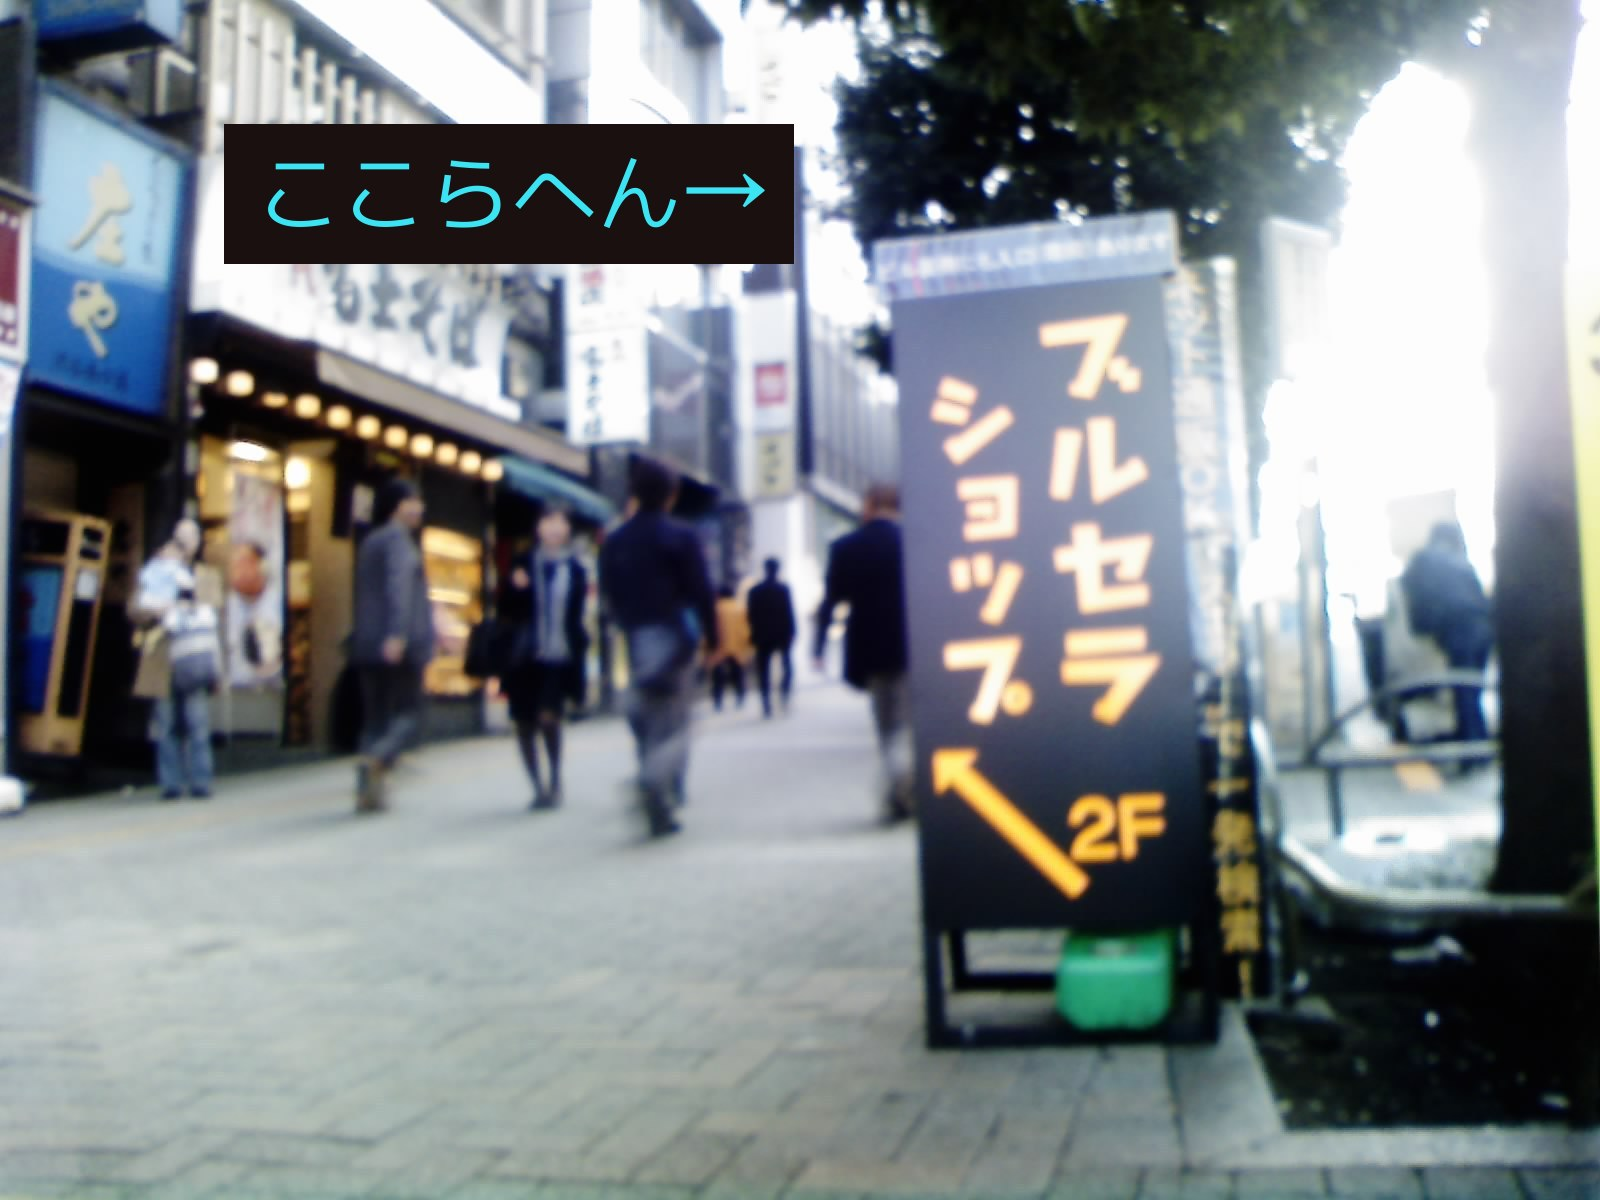
\includegraphics[width=1\hsize]{image200803/google-entry.jpg}
\end{frame}

\begin{frame}{}

前回初めて参加して、前回の内容がよかったから今回も参加しているという人挙手
\end{frame}


\section{DWN quiz}
\begin{frame}{Debian 常識クイズ}

Debian の常識、もちろん知ってますよね?
知らないなんて恥ずかしくて、知らないとは言えないあんなことやこんなこと、
みんなで確認してみましょう。

最近のアナウンス文書などから問題を出題しています。

\end{frame}

\subsection{問題}

%問題をコピペ

 \santaku
 {パッケージの品質確認に有用な次のツールのうち、lennyおよびsidから削除されたものは?}
 {lintian}
 {linda}
 {piuparts}
 {B}
 
 \santaku
 {リリースゴールの一つは、init.dスクリプトの実行順序を依存関係で決
 定できるようにすること。ところで、/etc/init.dにinitスクリプトを持つパッケージの数は?}
 {873}% パッケージの総数
 {857}% 対応済みパッケージの数
 {98}% 対応済みのパーセンテージ
 {A}
 
 \santaku
 {次のうち、Debian Installer Lenny Beta 1における改良点でないものは?}
 {NTPを用いた時刻合わせ}
 {volatileのサポートの追加}
 {Mac OS Xからのインストーラ起動のサポート}
 {C}
 
 \santaku
 {新たなDebianプロジェクトリーダー (DPL) に選ばれたSteve McIntyreが目標の一つに掲げているものは?}
 {Communications within the project}% 2008年DPLの標語の一つ
 {Make Debian sexy again}% 2007年DPLの標語の一つ
 {Welcoming people to the project}% 2006年DPLの2005年選挙での標語の一つ
 {A}
 
 \santaku
 {Debian Weekly Newsを復活させようというメールをdebian-devel-announceに流したのは?}
 {Martin Schulze}
 {Joey Hess}
 {Alexander Schmehl}
 {C}
 
 \santaku
 {lennyのリリースに関する現況として正しくないものは?}
 {GCC 4.3がデフォルトコンパイラとなり、それでコンパイルできないことがRCバグとなった}
 {lennyのリリースに向けて既に必須パッケージがフリーズされている}
 {デフォルトのsyslogデーモンをrsyslogに変更することが決定した}% まだ議論中
 {C}
 
 \santaku
 {dpkg 1.14.18で新たにいくつかのソースパッケージ形式がサポートされるようになったが、
 それらのうち次期デフォルトとされる「3.0 (quilt)」が持っていない機能は?}
 {ソースパッケージのupstream tarballとして複数のファイルを使用できる}
 {ソースパッケージのdiff.gzファイルを、適切に複数のパッチに分けてくれる}
 {ソースパッケージにDebian固有のバイナリファイルを挿入できる}
 {B}
 
 \santaku
 {今年のDPL選挙の投票率は?}
 {62.248\%{}}% 2000
 {53.084\%{}}% 2004
 {37.302\%{}}% 2008
 {C}
 
 \santaku
 {etchの次期ポイントリリースは「etch and a half」になるとされているが、
 そこに含まれる予定のLinuxカーネルのバージョンは?}
 {2.6.18}
 {2.6.24}
 {2.6.25}
 {B}
 
 \santaku
 {次の開発者のうち、新たにFTPマスターに任命されたのは?}
 {Sam Hocevar}
 {Joerg Jaspert}
 {James Troup}
 {B}
 
 \santaku
 {次の開発者のうち、Debian Marketing Teamのメンバーに任命されていないのは?}
 {Sam Hocevar}
 {Andreas Schuldei}
 {Moritz Muehlenhoff}
 {A}

 \santaku
 {Joerg Jaspert が DAM に任命されたのはSam Hocevar の任期の切れる何時間前か?}
 {24時間}
 {2時間}
 {-1時間}
 {B}

 \santaku
 {Software Design 2008年4月号155ページのgit-import-dscの事例にのっている
 パッケージ名は?}
 {ecasound}
 {pbuilder}
 {Windows Media Player}
 {A}

 \santaku
 {昨日 Debian 勉強会の参加メンバーで Debian Developer になったのはだれか?}
 {岩松}
 {小林}
 {Charles Plessy}
 {C}

\section{事前課題紹介}
\emtext{事前課題の紹介}
% pre work home work

\begin{frame}{事前課題問題}

\begin{enumerate}
 \item 「パッケージをつくってはまったこと」
 \item 「作ってみたいパッケージ」
 \item 「あなたはソースコードを管理しています。VCSを使うことでメリットを得ているのですが、使っていない友人にどう説明しますか?『○○○を使ったおかげで○○○になりました。なぜなら・・・。だからあなたもつかったほうがよいですよ。』」
\end{enumerate}

\end{frame}

% (query-replace "\\subsection" "\\end{frame}\\begin{frame}")
% (query-replace "\\subsubsection" "\\textbf")

\begin{frame}{Hiroyuki Yamamoto}

\textbf{「パッケージをつくってはまったこと・作ってみたいパッケージ」}

\begin{itemize}
 \item  パッケージをつくってはまったこと

 パッケージ自体を作ることにはあまりはまったことはないですが、最近、locale
 は UTF-8 が主流になってきていますが、仮想ターミナルで動く EUC-JP なプロ
 グラムを UTF-8 対応しようとした時、文字コードのバイト数が 2 バイト固定か
 ら 2-4 バイトに可変となっているため、コードを大幅にいじらないといけなく
 なっている場合があります。これからのユーザは UTF-8 でインストールするで
 しょうし、UTF-8 対応を無視もできなくて、困っています。あと、どうでも良い
 ことですが、dh-make がポリシー 3.7.3 に対応したテンプレを吐くようになる
 のはいつになるのかな?
\end{itemize}
\end{frame}\begin{frame}{Hiroyuki Yamamoto}
\begin{itemize}

 \item  作ってみたいパッケージ

 某巨大掲示板の専用ブラウザ kita2 をオフィシャルに上げようと思っていま
 す。アップストリームの作者には必要なファイルを入れてもらうよう交渉したと
 ころ。次期リリース待ち。
\end{itemize}

\end{frame}\begin{frame}{Hiroyuki Yamamoto}

\textbf{「あなたはソースコードを管理しています。VCSを使うことでメリットを得てい
るのですが、使っていない友人にどう説明しますか?『○○○を使ったおかげで○○○
になりました。なぜなら・・・。だからあなたもつかったほうがよいですよ。』」}

VCS は使っていません。是非、私にお薦めして下さい。

\end{frame}\begin{frame}{沖中}


\textbf{「パッケージをつくってはまったこと・作ってみたいパッケージ」}

今まで本格的にパッケージを作ったことがないので、はまったことはないです。
強いて言うなら、どこから手をつけていいか分かっていないところとか、
Makefile が分からないってことでしょうか。
既存のパッケージを参考にしようとしたのですが、何をやっているのか分からず、
とても難解に見えます。Makefile の記法を覚えるところから始めようと思っています。

私の作ってみたいパッケージは、探せば誰かが作っていたりするので、
これはぜひ私が!というものはないです・・・。更新が頻繁にされて、
パッケージかが追いついていないものを自前で作成する時がほとんどです。
あとは、自作のソフトくらいでしょうか。

\end{frame}\begin{frame}{akedo}

\textbf{「パッケージをつくってはまったこと・作ってみたいパッケー
   ジ」}

パッケージを作った事は無いので、作ってみたいパッケージと言う事で考えてみました。
インターネット公開サーバを個人で管理してたりすると、
あるとちょっと安心なのがkrfilter です。
これは iptables でフィルタするためのIPアドレスのリスト(設定スクリプト付き)です。
韓国(kr)だけでなく中国(cn)や台湾(tw)もあり、
個人的にはこれに .br とか .th も要りそうな気がしてます。
本格的なサーバには RBL(DNSBL)の方が良いかも知れません。

\end{frame}\begin{frame}{山本 琢}

\textbf{「あなたはソースコードを管理しています。VCSを使うことでメリットを得てい
るのですが、使っていない友人にどう説明しますか?」}

思いつくのはcvsですが、

\begin{itemize}
 \item  過去のソースコードを呼び出せる(個人での世代バックアップが不要)
 \item  変更履歴が参照できる(cvs log)
 \item  書いたソースとバージョンとの紐付けができる
\end{itemize}


\end{frame}\begin{frame}{やまね}

\textbf{「パッケージをつくってはまったこと」}
\begin{itemize}
 
 \item  ライセンス調整が大変

  開発元にお伺いを立てて変更を依頼したり、物によっては日本語ライセンスのみで英訳が必要だったりします。
  ライセンス解釈の問題があったりすることもありますし、non-free と扱われて reject を食らうことも。

 \item  pbuilder で build しないでアップロードしたら依存関係が変

  自分のマシンだと experimental が混じっているので、依存関係の問題が出たことが数回。
\end{itemize}

\textbf{「作ってみたいパッケージ」}

 すでに作りかけのパッケージがいくつも…。

\end{frame}\begin{frame}[containsverbatim]{前田}
\textbf{「パッケージをつくってはまったこと」}

技術的な話ではないのですが、ライセンスのとこで悩みます。GPLを採用していると謳っているソフトウェアでも、下記のような感じで書き換えていないのものがあると、本当にGPL採用しているのかと困ってしまいます。

\begin{commandline}
 > one line to give the program's name and an idea of what it does.
 > Copyright (C) yyyy name of author
\end{commandline}

パッケージをつくっても、自分で使う為だけにしかやらないのはそういうところが、面倒だからなんだと思います。きっと。

\end{frame}\begin{frame}{本庄}
\textbf{パッケージをつくってはまったこと}
はまったわけではないですが、debian/controlなどのdebian/以下をど
のように書くべきか、いつも悩みます。

\textbf{作ってみたいパッケージ}
HTML::DOMboというCPANモジュールが便利なのですが、CPANモジュール
ということ、名前がちょっと怪しいということで微妙です。


\end{frame}\begin{frame}{堀内寛己}

勉強会/懇親会には欠席の予定ですが、課題だけ。

\textbf{「あなたはソースコードを管理しています。VCSを使うことでメリットを得てい
るのですが、使っていない友人にどう説明しますか?」}

もう語りつくされたことだと思いますが、CVS以上のVCSなら、
「いつどこでバグが入りこんだか突き止めやすい」ということでしょうか。
たとえテスト駆動開発をしていたとしても、
回帰テストをすり抜けるバグというのもありうるわけで、
その点でも、いつまでも重要なメリットだと思います。

\end{frame}\begin{frame}[containsverbatim]{濱野}

\textbf{パッケージをつくってはまったこと・作ってみたいパッケージ}

\verb!LD_PRELOAD! を使うようなパッケージを作ろうとした時に、共有ライブラリにバー
ジョンが付いているからダメというような lintian の警告ではまりました。
これに限らず、lintian には良く解らない理由で何度も何度も怒られました。
ポリシーを理解していないからなので自業自得のような気がします。

\end{frame}\begin{frame}[containsverbatim]{濱野}

\textbf{「あなたはソースコードを管理しています。VCSを使うことでメリットを得てい
るのですが、使っていない友人にどう説明しますか?」}
今頃になって CVS で管理していたいろいろなモノを git に移行しています。
git を使ったおかげでディレクトリの移動が簡単に出来るようになりました。
遠慮せずにローカルレポジトリにガシガシコミットすることも出来ます。
でも時々、更新されない CVS のキーワード \verb!$Id:$! などを見るたび物悲しくな
ります。

\end{frame}\begin{frame}{日比野 啓}

\textbf{パッケージをつくってはまったこと}

あるライブラリをパッケージ化したときに、
ちょっとパッチを当てる必要があって修正を行ないました。
そのライブラリのMakefileではコンパイル単位のソースファイルがいくつかのディレクトリに分散して置けるようになっていて、
Makefileはそのディレクトリを順番にソースファイルを探しにいくように(GNU make の vpath)なっていたのです。
修正前のファイルをたまたま vpath の手前にあるディレクトリに置きっぱなしにしていたために
コンパイルしなおしても修正が反映されない原因がわからなくてハマりました。

\end{frame}\begin{frame}{日比野 啓}

\textbf{作ってみたいパッケージ}

OCaml言語のネイティブコンパイラに動的ライブラリをビルドする機能がマージされたのですが、
その機能が入ったコンパイラおよび、ライブラリ一式をDebian化して使えるようにしたいです。
リリース版のバージョンに入るにはもうしばらくかかりそうなので。

\end{frame}\begin{frame}{藤沢理聡}

\textbf{VCSを使うことでメリットを得ているが、使っていない友人にどう説明す
るか}

 研究室で大きなシステムを組むことになったとき、VCSは欠かせません。実際に作 
成するシステムのプログラム群の管理はもちろんのこと、ドキュメントなどの関係 
者全員で共有したいデータの管理にも有効です。特に研究室などでは、メンバーが 
集まる時間がなかなか合わなかったり、人によってはリモートアクセスで開発等を 
行ったりするため、データが更新されるタイミングがわかりづらいこともありま 
す。そのような場合に、VCSを用いることで最近変更された箇所などを把握しやすい 
ことは、システム開発を進める上で大きな利点です。

\end{frame}\begin{frame}{jitsukata}

\textbf{パッケージをつくってはまったこと}

はまったのとは少し違いますが、パッケージを作成するのに複数のスタイルがあることに混乱しました。
debhelper、CDBS、dpatch、dbs、quilt、yadaの使い分け、関連性がよく分かりません。
それぞれメリット・デメリットがあると思いますが、複数のスタイルがあることで、
何を使えば良いのか分かりにくいと感じました。

\end{frame}\begin{frame}{キタハラ}

\textbf{「パッケージをつくってはまったこと・作ってみ
たいパッケージ」}

debianのパッケージに関しては、今年の3月1日に
試みたのが初めてで、講義の速度についていけず、未完
に終わったという恥ずかしい経験しかないもので、何を
書いてよいのやら・・・。

無難に「自作のプログラムをパッケージにしてみた
い」と書こうと思ったが、最近プログラムを書いていな
かった。(某OS上ではマクロとかスクリプトとかを
山ほど書いては捨てているのですが・・・) 

\end{frame}

\emtext{2008年計画}

\begin{frame}{2008年計画}

{\scriptsize
\begin{enumerate}
 \item 新年会「気合を入れる」
 \item Open Source Conference Tokyo (3/1)
 \item データだけのパッケージを作成してみる、
       ライセンスの考え方 (David Smith)
 \item バイナリ一つのパッケージを作成してみる (吉田@板橋)\\
       バージョン管理ツールを使いDebianパッケージを管理する(git)\\
       アップストリームの扱い(svn/git/cvs)(岩松 信洋さん)
 \item バイナリの分けたパッケージの作成。(前田さん)\\
       バイナリの分け方の考え方、アップグレードなどの運用とか。
 \item パッケージ作成(dpatch/debhelperで作成するパッケージ)(小林儀匡さん)\\
       man の書き方(roff or docbook)(でんさん)
 \item パッケージ作成(kernel patch、kernel module)
       、Debconf発表練習
 \item Debconf アルゼンチン、共有ライブラリパッケージ作成

 \item Open Source Conference Tokyo/Fall、
       デーモン系のパッケージの作成、latex、 emacs-lisp、フォントパッケージ
 \item パッケージの cross-compile の方法、amd64 上で i386 のパッケージと
       か、OSC-Fall報告会、Debconf報告会
 \item 国際化 po-debconf / po化 / DDTP
 \item 忘年会
\end{enumerate}
}
\end{frame}

\emtext{バイナリ一つだけのパッケージを作成してみる}
\emtext{バージョン管理ツールを使い Debian パッケージを管理する Git編}
\emtext{アップストリームの VCS と付き合う}
\emtext{Nexenta Core Platformを使ってみる}

\section{Nexenta Core Platformを使ってみる}

\begin{frame}{Nexenta Core Platform}
\begin{itemize}
 \item  OpenSolaris \url{http://www.opensolaris.org/os/}
 \item  Nexenta \url{http://www.nexenta.org/os}:
	Debian GNU/Linux のパッケージングシステムを OpenSolarisに移植
 \item Nexenta Core Platform が2008年2月にリリース
\end{itemize}

\end{frame}

\begin{frame}[containsverbatim]{起動コマンド}
\begin{commandline}
$ qemu-system-x86_64 -hda nexenta.cow \
 -cdrom  nexenta-core-platform_1.0-b82_x86.iso \
 -boot d \
 -m 512 
\end{commandline}
\end{frame}


\begin{frame}{Nexenta画面写真} 
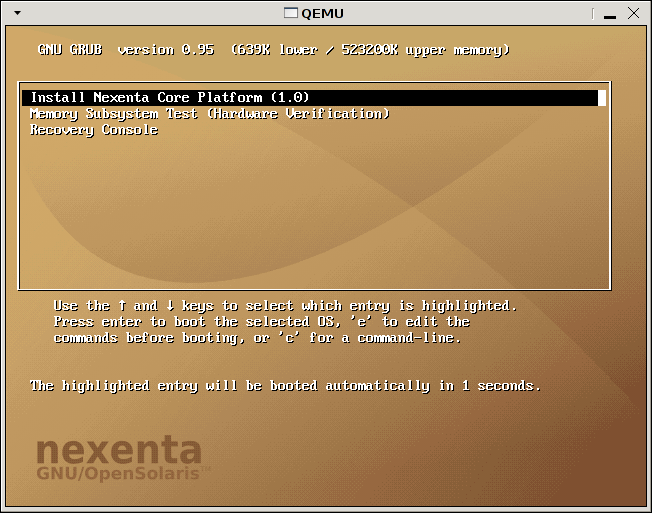
\includegraphics[width=1.0\hsize]{image200804/nexenta1.png}
\end{frame}\begin{frame}{Nexenta画面写真} 
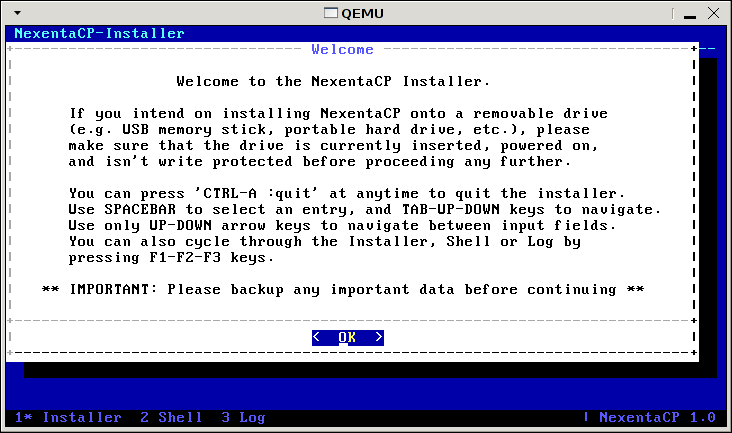
\includegraphics[width=1.0\hsize]{image200804/nexenta2.png}
\end{frame}\begin{frame}{Nexenta画面写真} 
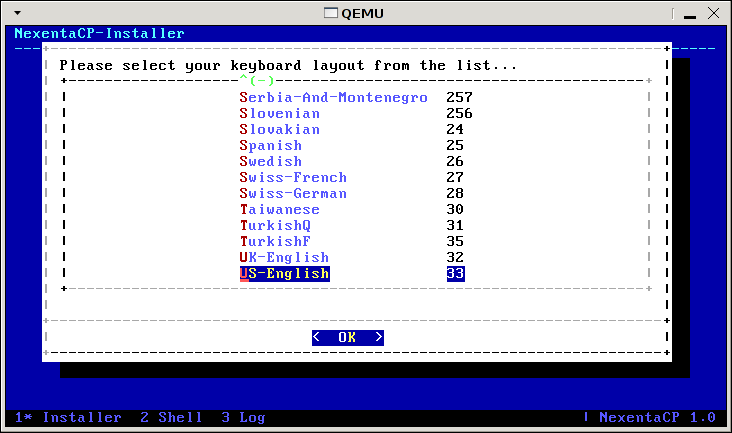
\includegraphics[width=1.0\hsize]{image200804/nexenta3.png}
\end{frame}\begin{frame}{Nexenta画面写真} 
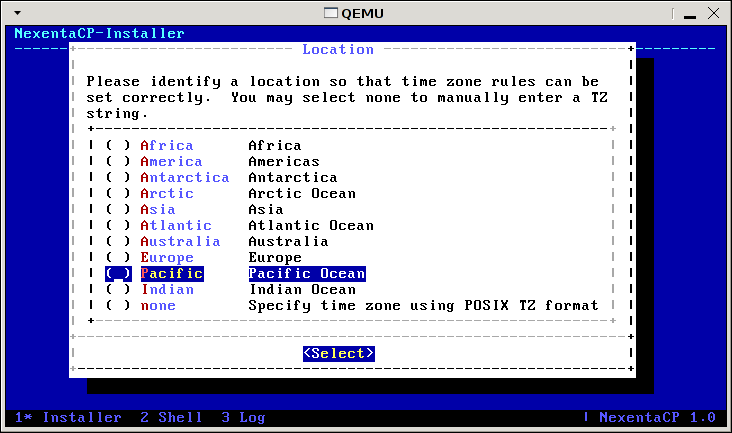
\includegraphics[width=1.0\hsize]{image200804/nexenta4.png}
\end{frame}\begin{frame}{Nexenta画面写真} 
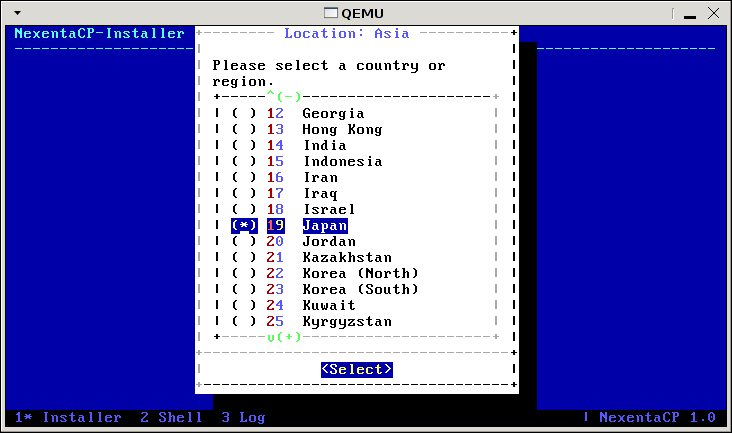
\includegraphics[width=1.0\hsize]{image200804/nexenta5.png}
\end{frame}\begin{frame}{Nexenta画面写真} 
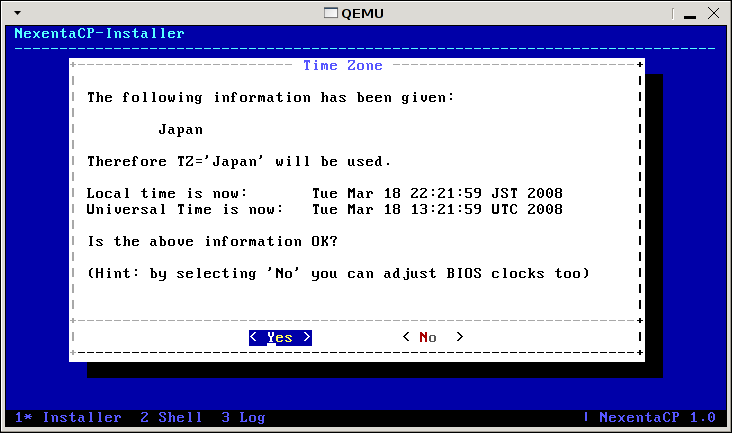
\includegraphics[width=1.0\hsize]{image200804/nexenta6.png}
\end{frame}\begin{frame}{Nexenta画面写真} 
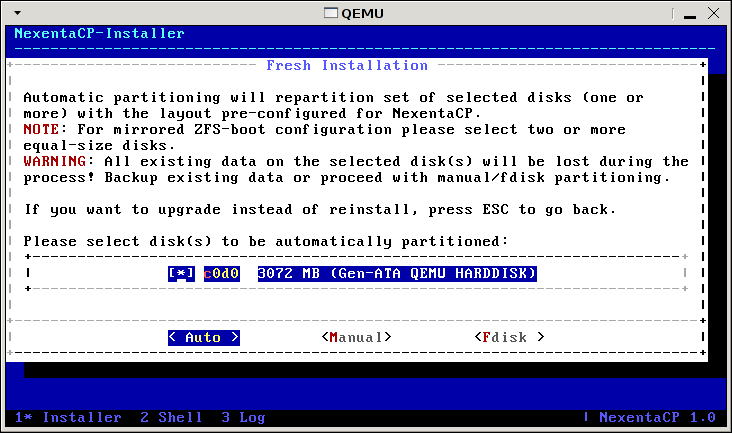
\includegraphics[width=1.0\hsize]{image200804/nexenta7.png}
\end{frame}\begin{frame}{Nexenta画面写真} 
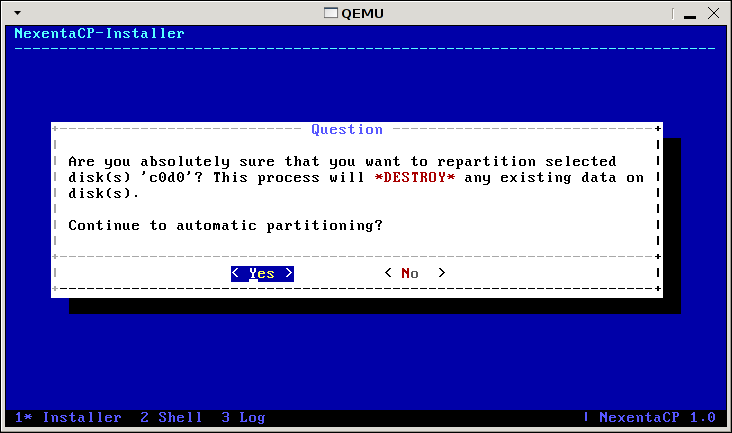
\includegraphics[width=1.0\hsize]{image200804/nexenta8.png}
\end{frame}\begin{frame}{Nexenta画面写真} 
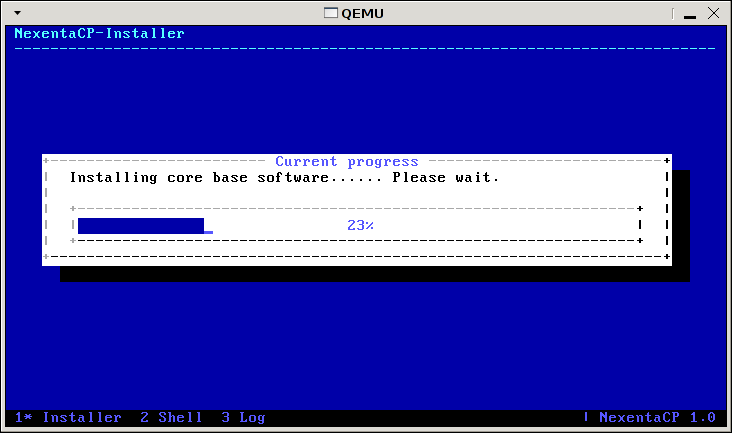
\includegraphics[width=1.0\hsize]{image200804/nexenta9.png}
\end{frame}\begin{frame}{Nexenta画面写真} 
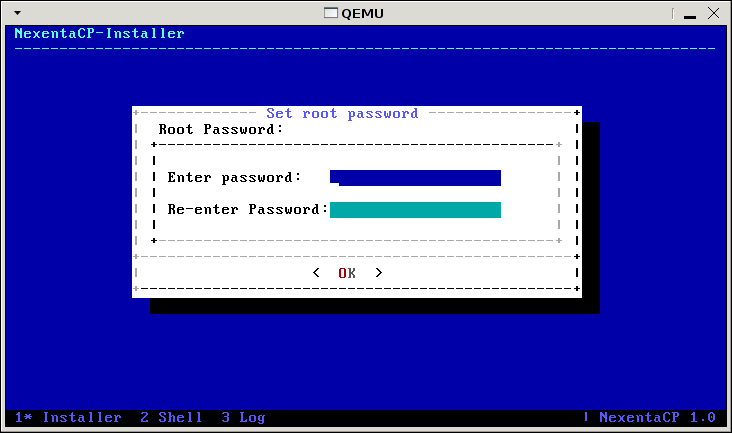
\includegraphics[width=1.0\hsize]{image200804/nexenta10.png}
\end{frame}\begin{frame}{Nexenta画面写真} 
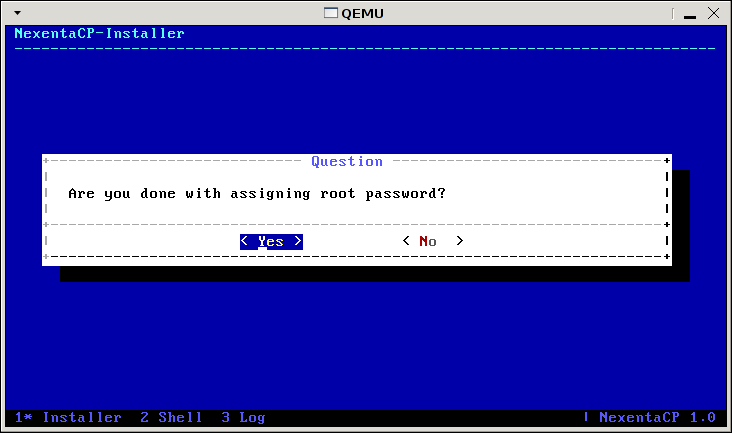
\includegraphics[width=1.0\hsize]{image200804/nexenta11.png}
\end{frame}\begin{frame}{Nexenta画面写真} 
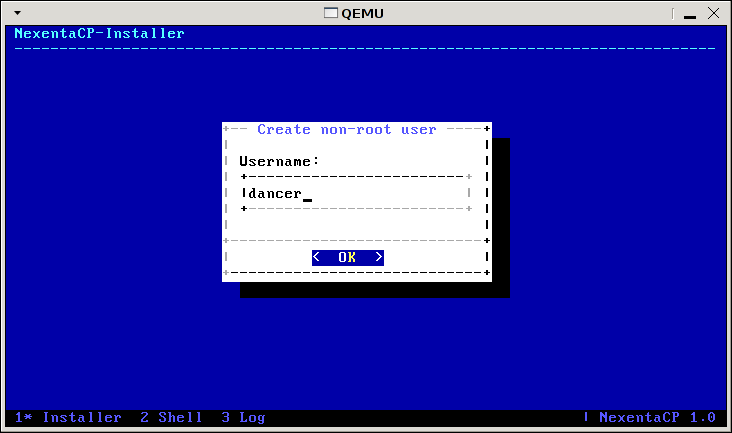
\includegraphics[width=1.0\hsize]{image200804/nexenta12.png}
\end{frame}\begin{frame}{Nexenta画面写真} 
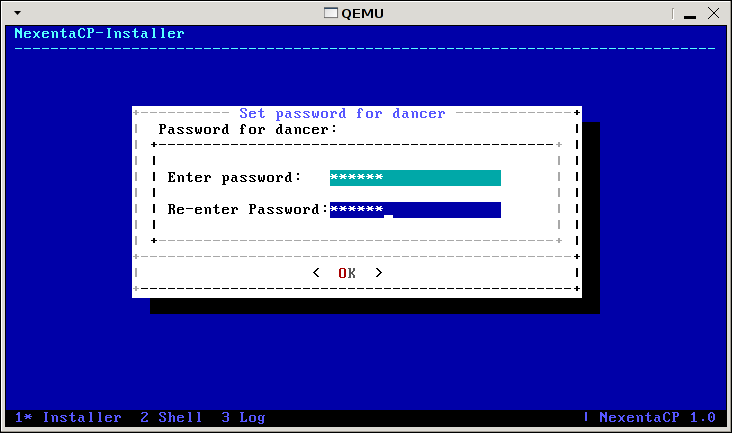
\includegraphics[width=1.0\hsize]{image200804/nexenta13.png}
\end{frame}\begin{frame}{Nexenta画面写真} 
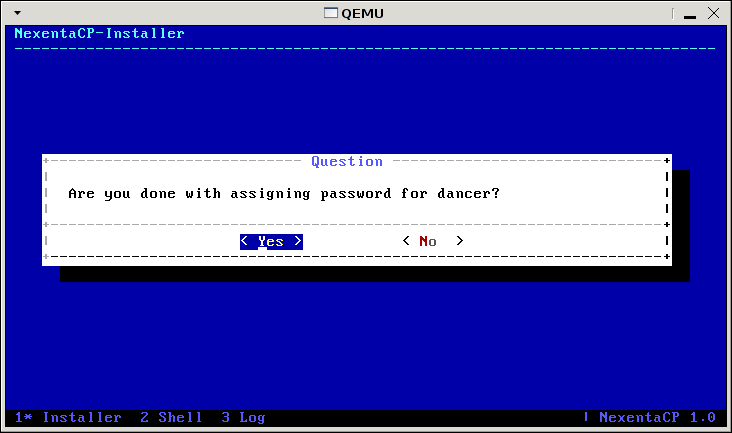
\includegraphics[width=1.0\hsize]{image200804/nexenta14.png}
\end{frame}\begin{frame}{Nexenta画面写真} 
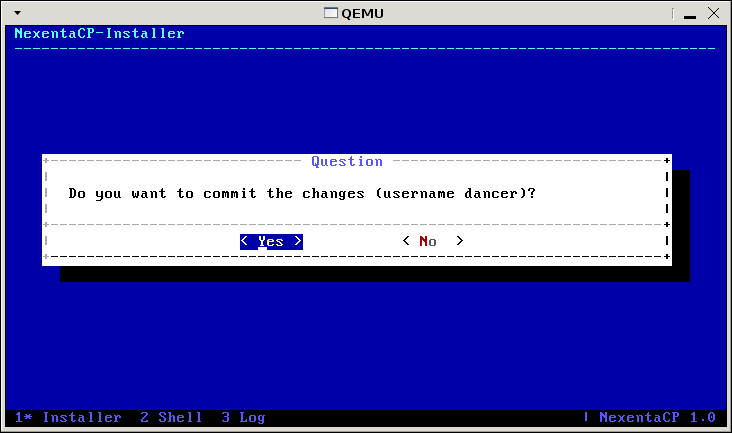
\includegraphics[width=1.0\hsize]{image200804/nexenta15.png}
\end{frame}\begin{frame}{Nexenta画面写真} 
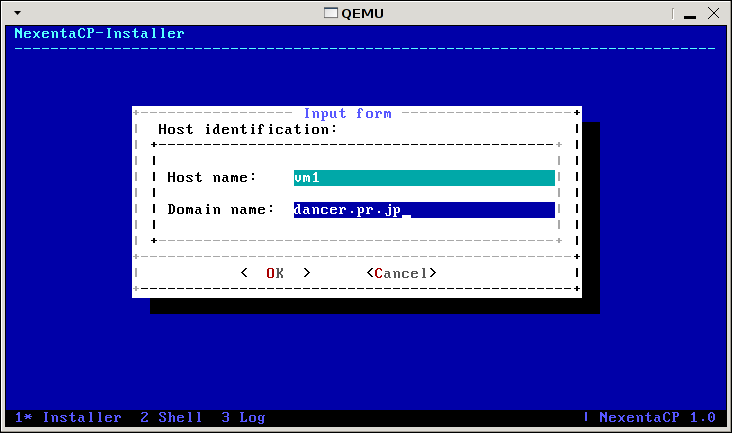
\includegraphics[width=1.0\hsize]{image200804/nexenta16.png}
\end{frame}\begin{frame}{Nexenta画面写真} 
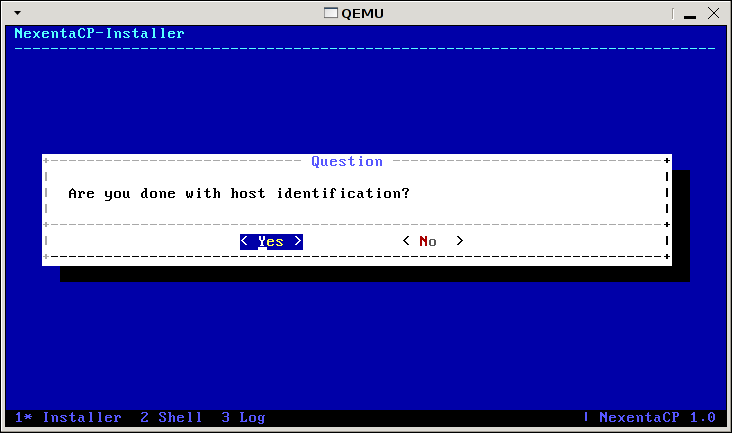
\includegraphics[width=1.0\hsize]{image200804/nexenta17.png}
\end{frame}\begin{frame}{Nexenta画面写真} 
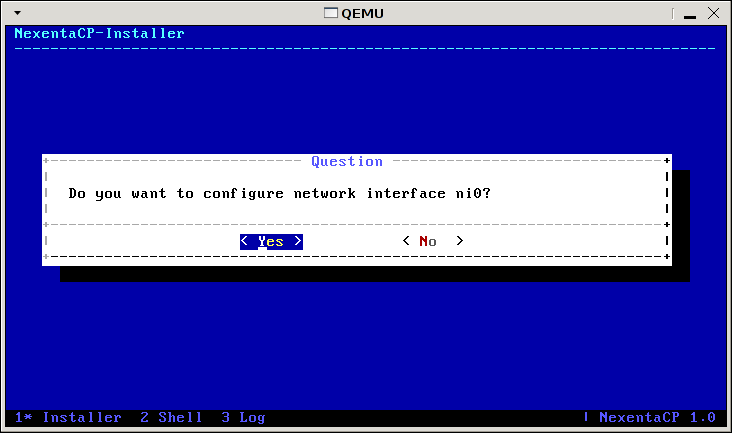
\includegraphics[width=1.0\hsize]{image200804/nexenta18.png}
\end{frame}\begin{frame}{Nexenta画面写真} 
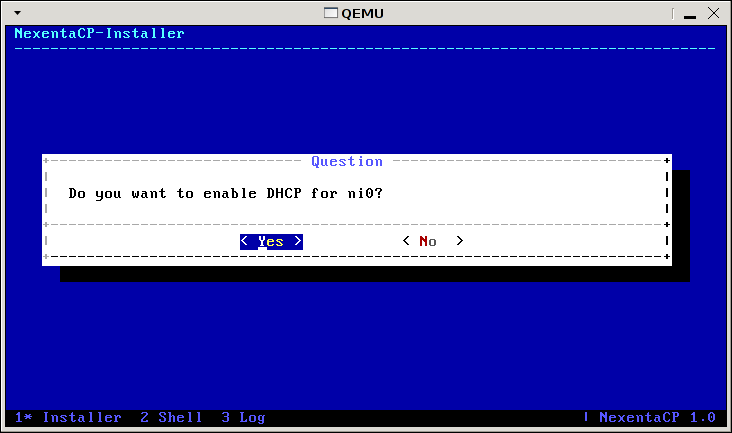
\includegraphics[width=1.0\hsize]{image200804/nexenta19.png}
\end{frame}\begin{frame}{Nexenta画面写真} 
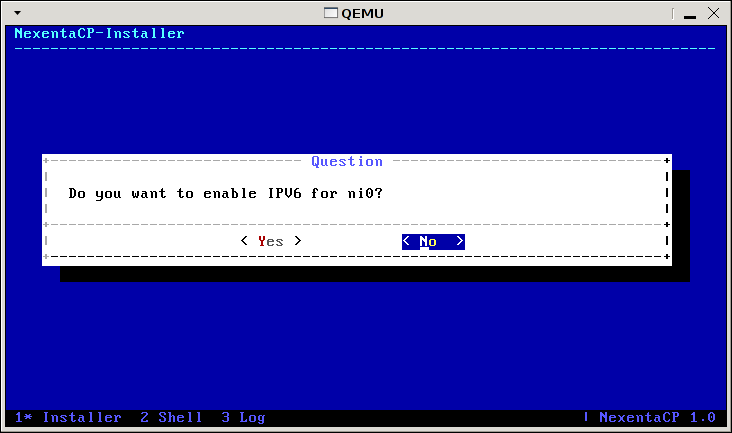
\includegraphics[width=1.0\hsize]{image200804/nexenta20.png}
\end{frame}\begin{frame}{Nexenta画面写真} 
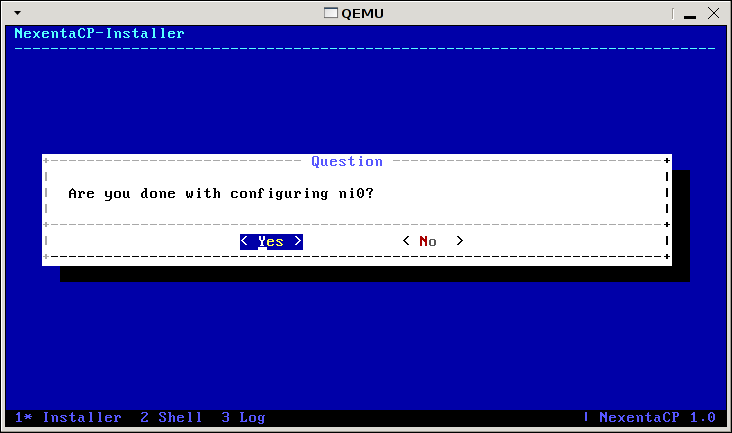
\includegraphics[width=1.0\hsize]{image200804/nexenta21.png}
\end{frame}\begin{frame}{Nexenta画面写真} 
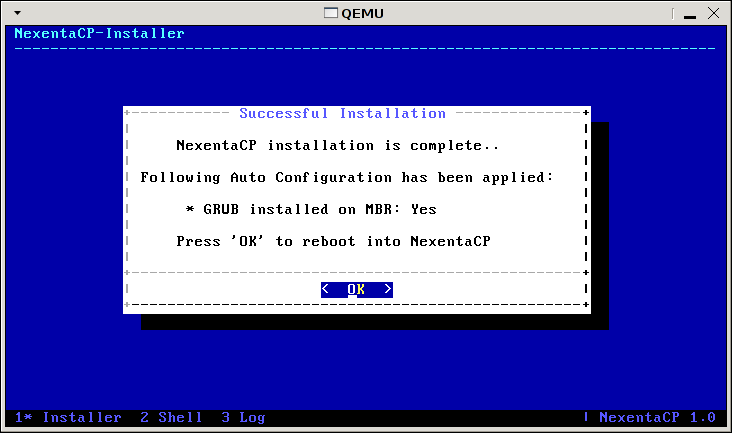
\includegraphics[width=1.0\hsize]{image200804/nexenta22.png}
\end{frame}\begin{frame}{Nexenta画面写真} 
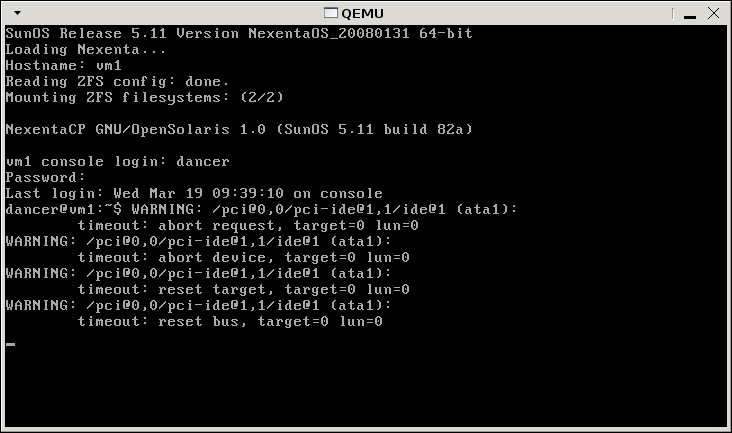
\includegraphics[width=1.0\hsize]{image200804/nexenta23.png}
\end{frame}

\begin{frame}{宴会場所}
\begin{center}
 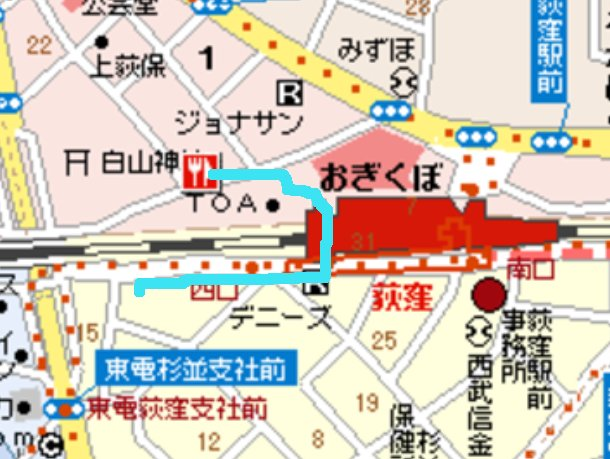
\includegraphics[width=0.5\hsize]{image200804/enkaimap.jpg}
\end{center}

\begin{itemize}
 \item 宴会場所\\
       本日の宴会は「駒忠」です。\\
       参加者はB1Fに集合し、全員で移動しましょう。
 \item 片付け\\
       部屋を片付けるのにご協力ください。
\end{itemize}

\end{frame}

\end{document}

;;; Local Variables: ***
;;; outline-regexp: "\\([ 	]*\\\\\\(documentstyle\\|documentclass\\|emtext\\|section\\|begin{frame}\\)\\*?[ 	]*[[{]\\|[]+\\)" ***
;;; End: ***
